\subsection{Les classes d'agents}
\begin{frame}
\frametitle{Modèle}
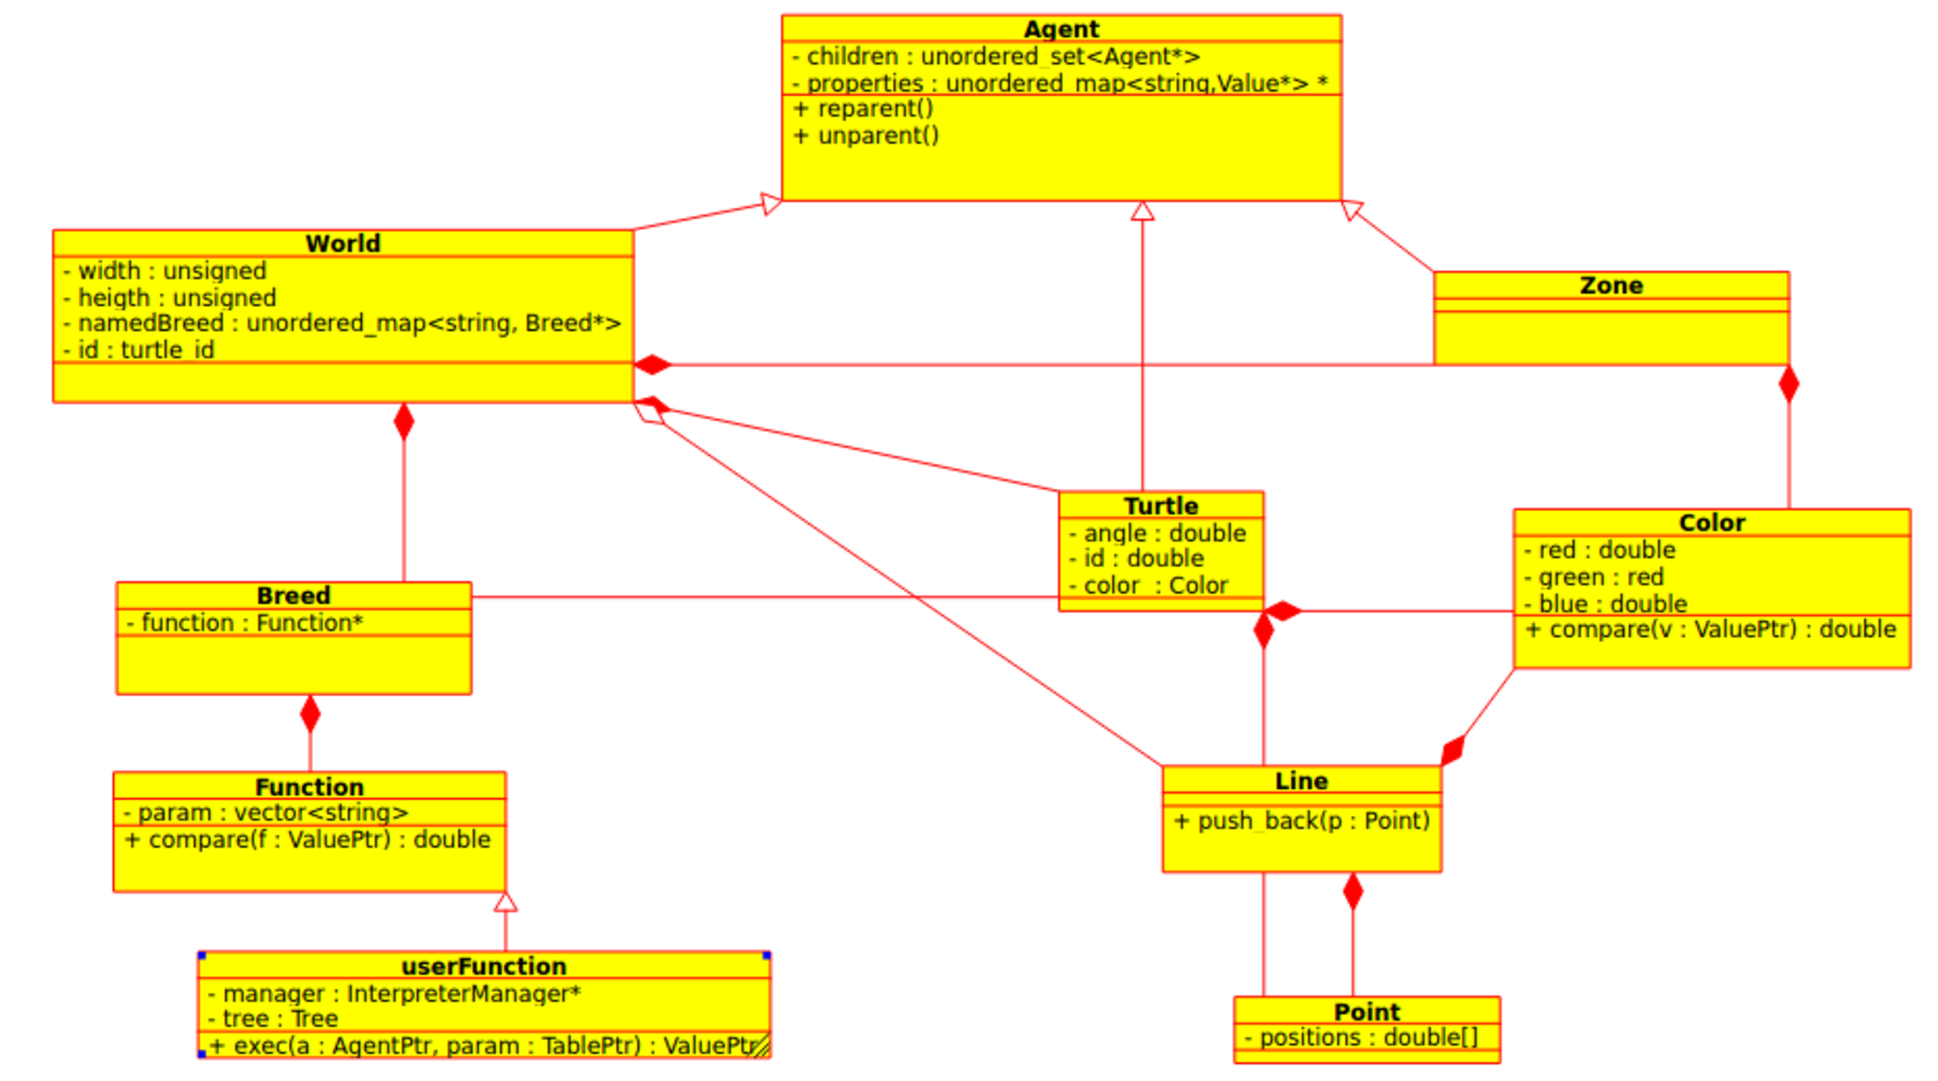
\includegraphics[scale=0.31]{doc/Presentation/image/agents.pdf}
\end{frame}

\note{diagramme=modèle à l'état final.\\
version 1 : turtle point, line, world. le but étant de pouvoir dessiner une ligne. Le monde stocke les lignes, chaque tortue a une ligne\\
version 2 : classes agent(regroupe comportement) et breed(nommée ou pas), ajout des fonctions, qui stocke un arbre abstrait, contenant le code de la fonction déjà analysé;
 Ajout des mutexs pour la sureté des accés aux attributs\\
version 3 : les communications : zones propriétés et tortues send, recv...;
ajouts des pointeur intelligents pour limité les fuites mémoires sur classes principales\\
 export : méthode dans chaque agent; utilisation de json spirit pour l'écriture du json\\
ajout user function, qui correspond au fonction crée par l'utilisateur, classe spé de function
Utilisation de cpp unit pour les tests unitaires : une classe pour chaque test
}

\subsection{Les types}
\begin{frame}
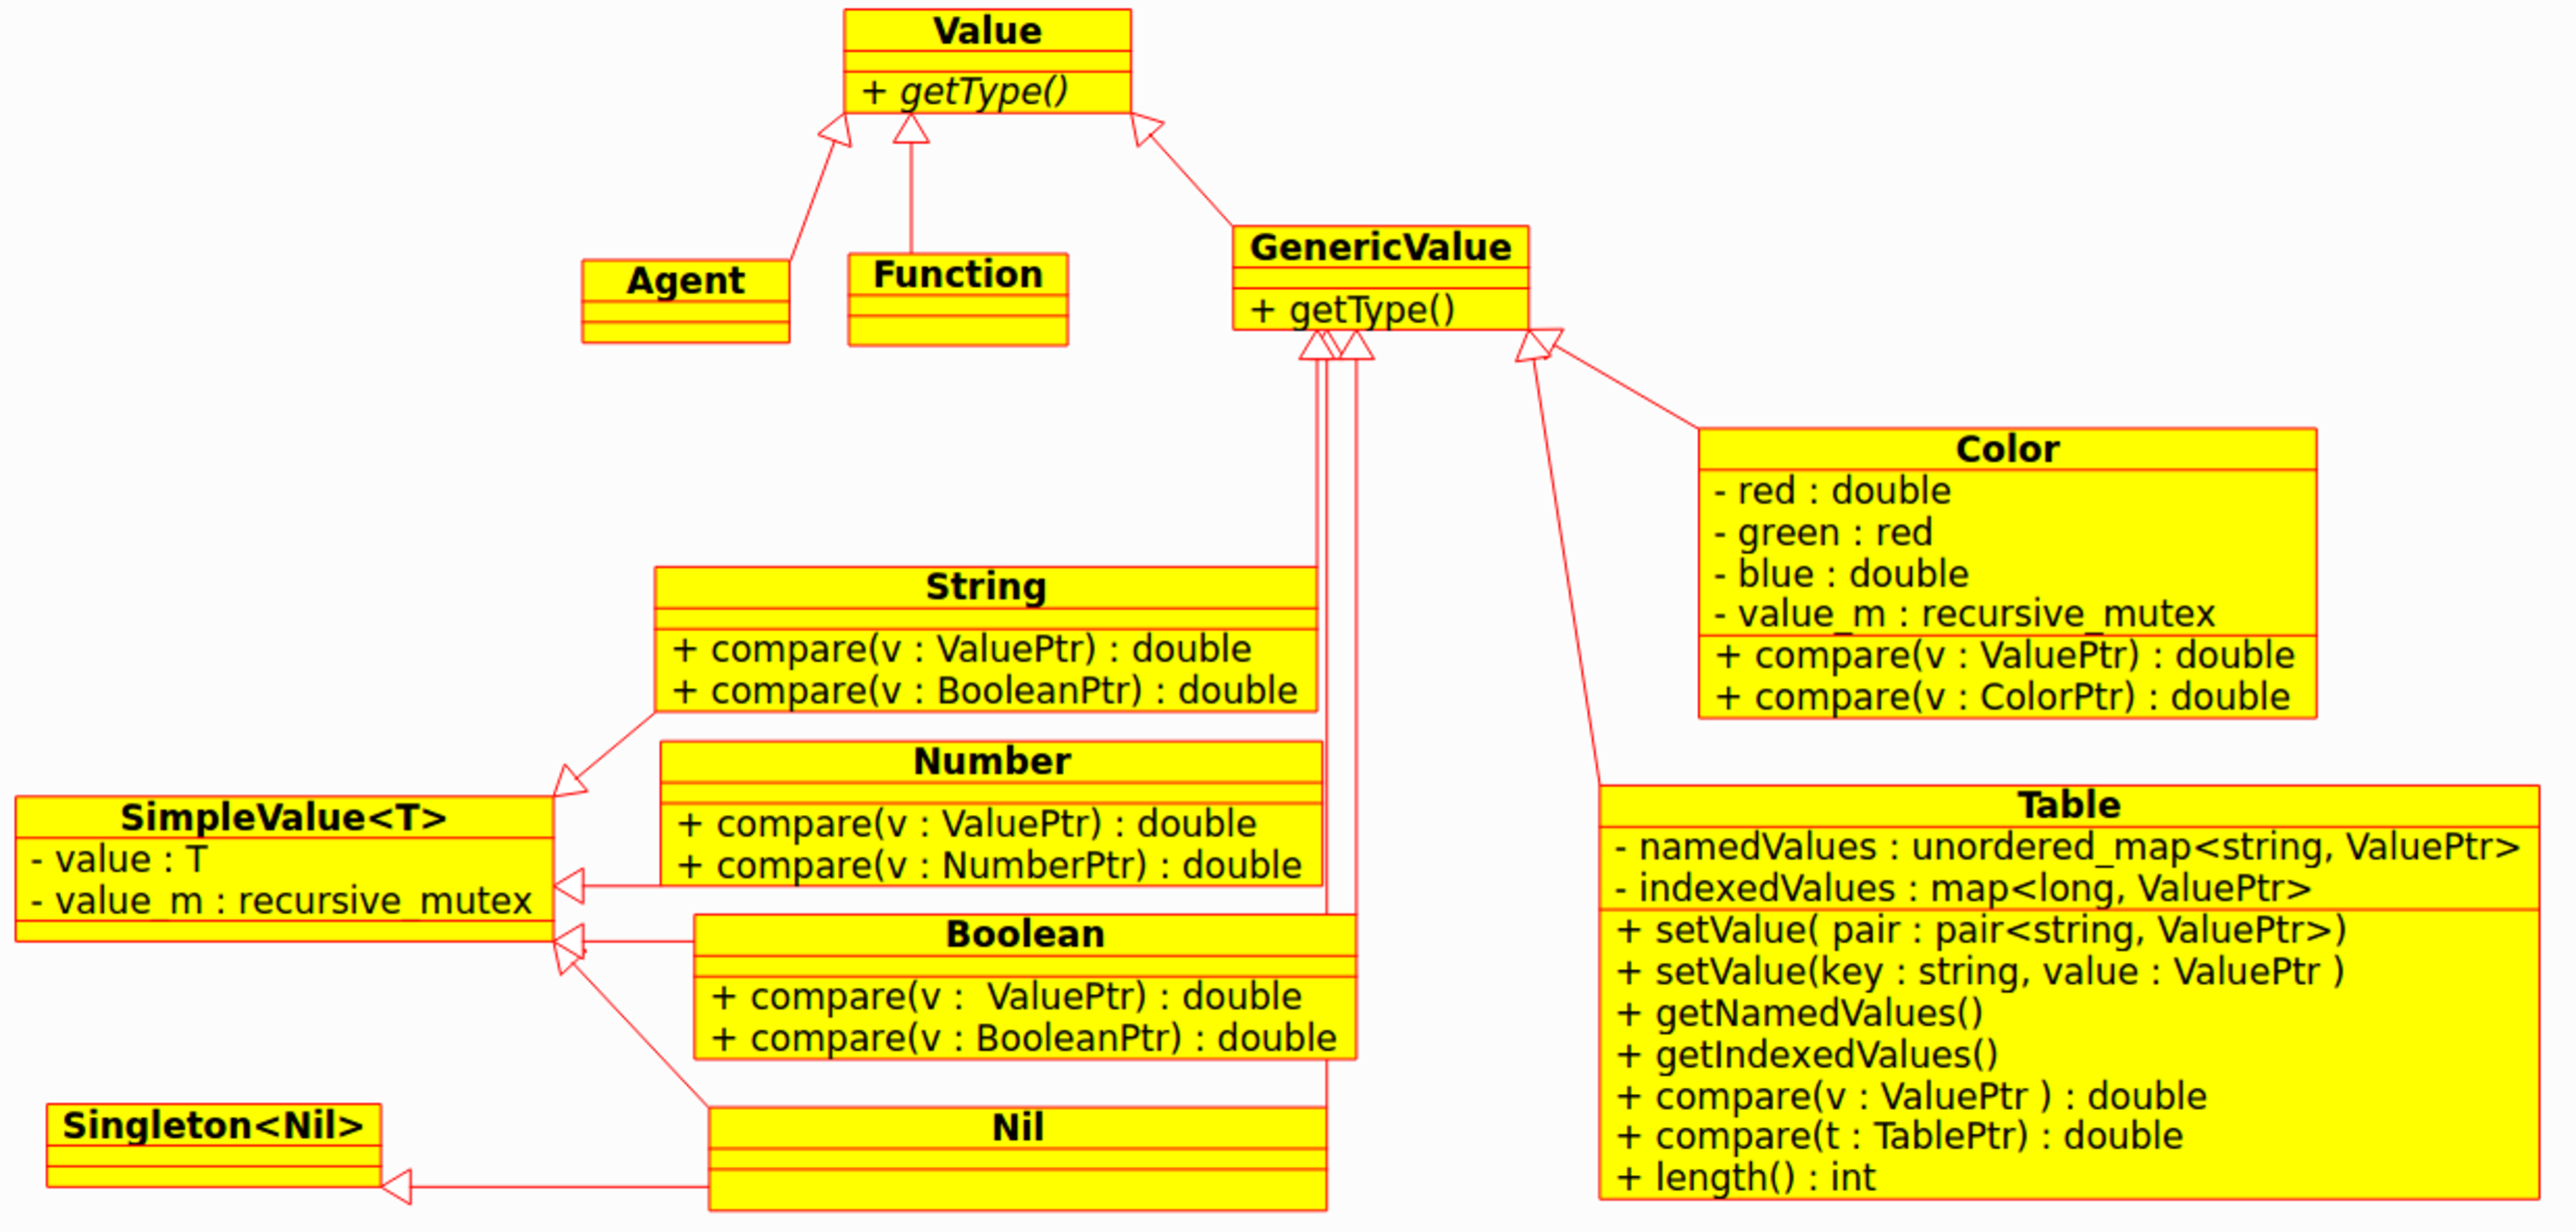
\includegraphics[scale=0.27]{doc/Presentation/image/types.pdf}
\end{frame}
\note{1er sprint : color nil et value\\
2eme : compléxifié avec simple value<Type T> pour les mutexs, généric value qui hérite de value pour spécialisé la méthode getType, value nos paramétrable car sinon ca créee des classes différentes \\
4eme : table et mutex recursifs
}
